% !TeX root = ../main.tex

\begin{survey}
\label{cha:survey}

\title{
  Bound Analysis : A Brief Overview
}

\maketitle

Automatic methods for computing bounds on the resource consumption of programs are an active research field. Bound analysis, or complexity analysis, tells the potential worst-case scenario complexity of a program, and is thus useful for predicting performance. This literature review briefly documents some of the recent works on automated bound analysis. 

\tableofcontents

\section{Introduction}

Bound analysis is a branch of program analysis which attempts to determine the \textit{resource consumption} of a given program. The result is a symbolic formula over the input parameters of the program. Basically, it's the problem of deciding how many steps a Turing machine can take at most, given any input.

This is obviously an undecidable problem, since if it's decidable, we can use the decision procedure to decide the famous halting problem:

\begin{theorem}[Turing 1936\cite{turing_computable_1937}, Halting Problem]
  Given a Turing machine M and input word w, it is undecidable if M will halt on w.
\end{theorem}

Bound analysis nowadays is usually based upon \textit{termination analysis}{\cite{cook_proving_2011}}, which is the problem of deciding if a program always terminates on any input. Termination analysis is even not semi-decidable. In fact, it is neither RE nor co-RE.

The undecidability of this problem implies that, any sound method to bound analysis must be incomplete. That is, there is always an input on which the method cannot give a result. Current techniques often presume a special subset of program features that make the program class decidable (for termination), one of which is simple linear loop program. Even so, proof of a program to be terminating is not always directly appliable to bound analysis.

There are many automated bound analysis methods in the literature. We mainly focus on two methodologies in the following sections.

\section{Preliminary}

We briefly introduce some concepts here.

\begin{definition}[Transition System]
  Formally, a {\textbf{transition system}} is a pair $(S, R, I)$ where $S$ is a set of states and R is a relation of state transitions (i.e., a subset of $S \times S$). A transition from state p to state q, i.e. $(p, q) \in R$, is written as $R(p,q)$. $I$ is the set of initial states.
\end{definition}

Transition system can be seen as the most low-level model we use. On the other hand, a program has higher abstraction via CFG:

\begin{definition}[Program]
  A program is a CFG $(L, \tau, l_0)$, where L is the set of program locations, $\tau \subseteq L \times R \times L$ is the transition relation, where $R \subseteq S \times S$, and $l_0$ is a distinguished initial location.
  
  A program state is $(l, s)$ where l is a location and s is a memory state.
  
  A computation is a sequence $(l_0, s_0), (l_1, s_1), \ldots$ where for each i > 0, there is $(l_i, \rho, l_{i + 1}) \in \tau$ and $\rho (s_i, s_{i + 1})$.
  
  A program is said to be terminating if there is no infinite computation.
\end{definition}

If all the variables of a program are natural number, we can get a special case : the lossy VASS.

\begin{definition}[Lossy Vector Addition System with States]
  A VASS is a program with a fixed set of variables $\{ x_1, \ldots, x_n \}$. The edge is denoted as $x' \leqslant x + d$ with $d \in \mathbb{N}^n$.
\end{definition}

Note that variables in VASS are natural numbers, so there is a lower bound 0 for them.

\begin{definition}[Loop]
  Let G = (V, E) be a directed graph with a unique entrypoint such that all nodes are reachable from the entry point. A node a dominates a node b, if every path from entry to b includes a. An edge l1 $\rightarrow$ l2 is a back edge, if l2 dominates l1 . G is reducible, if G becomes acyclic after removing all backedges. A node is a loop header, if it is the target of a back edge. The (natural) loop of a loop header h in a reducible graph is the maximal set of nodes L such that for all x $\in$ L (1) h dominates x and (2) there is a back edge from some node n to h such that there is a path from x to node n that does not contain h.
  
  A loop-path $\pi$ is a simple cyclic path, which starts and ends at some loop header l, and visits only locations inside the natural loop of l.
\end{definition}

\begin{definition}[Inductive Invariants]
  An invariant map Q maps program locations l to state formulas $I_l$.
  
  For a program C, Q is inductive if for any $(l, l', \rho) \in \tau_C$, the following holds: 
  
  \[ \forall s, s', I_l (s) \wedge \rho (s, s') \rightarrow I_{l'} (s') \]
  
\end{definition}

\section{Control Flow Abstraction}

The tool \textit{Loopus} {\cite{sinn_simple_2014, sinn_complexity_2017, sinn_difference_2015}} utilizes an automated method of bound analysis. The algorithm is composed of 4 steps:

\begin{enumerate}
  \item Abstracting a program into a VASS
  
  \item Control Flow Abstraction, which 'flatten' the VASS and merge the loops
  
  \item Ranking function generation, which proves the VASS to be terminating
  
  \item Bound Analysis, which computes a bound for every transition.
\end{enumerate}

The first step is neglected here. The second step, \textit{control flow abstraction}, basically analysizes the program and find all the loop paths. It then transform the original VASS into a singleton state transition system with many transtion on it. The algorithm is as follows:

\begin{figure}
    \centering
    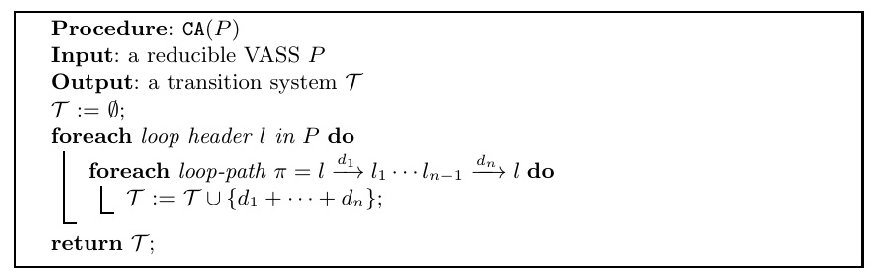
\includegraphics[width=0.8\linewidth]{survey1.pdf}
    \caption{control flow abstraction}
\end{figure}

Now we get a transition system with a single state where each transition stands for a loop path. In {\cite{sinn_simple_2014}}, the transition system is then analysized and a ranking function is generated. The ranking function is lexicographic, and each component of the ranking function is a variable among $x_1, \ldots, x_n$. In general, a ranking function could be any valid expression, thus it's possible that a single-variable ranking function does not exist. However inexpressive, this generation algorithm is relatively complete.

The last step of the analysis gives the actual bound. Suppose the transtion $\rho$ has the ranking function component x, then $\rho$ can be executed $\tmop{Init} (x)$ times if no other transitions increase x. So we have to take
other transitions into account. The algorithm is as follows:

\begin{figure}
    \centering
    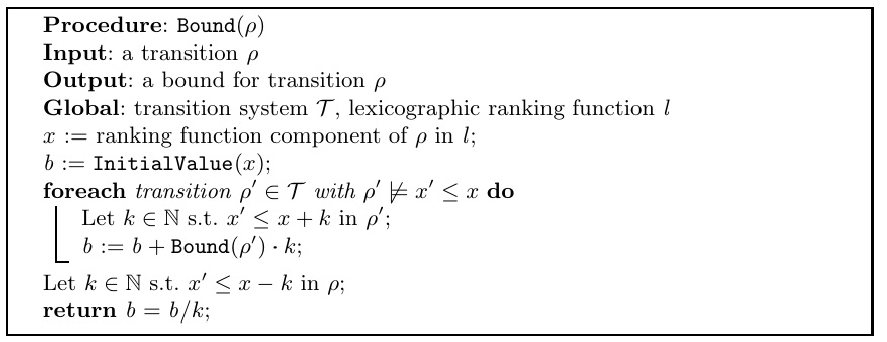
\includegraphics[width=0.8\linewidth]{survey2.pdf}
    \caption{algorithm to compute the bound}
\end{figure}

Now that a bound for each transition is obtained, we simply add them to get
the final bound.

\section{Compute WCCC using Ehrhart polynomials}

The tool \textit{Rank}{\cite{alias_multi-dimensional_2010}} gives a novel way of computing \textit{worst-case computational complexity}(WCCC). The method also generate (lexicographic) ranking function first. However, different to the method mentioned above, the ranking function can be any affine expression. Besides, since no control flow abstraction are used, the CFG is general. Thus every location in the graph is assigned a ranking function, in other words, the ranking function is inductive.

Consider any trace $(l_0, x_0), \ldots, (l_p, x_p)$, by definition of ranking function, we have $r (l_i, x_i) < r (l_{i + 1}, x_{i + 1})$, thus, every states in the trace must be distinct.

Hence the length of a trace is bounded by:

\[ \tmop{WCCC} \leqslant \# \bigcup_k r (k, P_k) \leqslant \sum_k \#r (k, P_k)
\]

The goal here is to compute $r (k, P_k)$ for each location k, where $P_k$ is the inductive invariant at location k. Basically, we find the number of points in the intersection of $\mathbb{Z}^n$ and the image of a polyhedron.

The authors use Smith normal form and Ehrhart polynomials to compute this ordinal. Suppose $r (k, x) = R x + r$, we compute $R = U S V$, where U and V are unimodular and $S = \left[ \begin{array}{cc}
  D & 0\\
  0 & 0
\end{array} \right]$ where D is diagonal positive matrix of the same rank as R. Then $\#V$ is a slight overapproximation of $\#r (k, P_k)$. The number of integer vector in V is obtained using Ehrhart polynomials.

\bibliographystyle{unsrtnat}
\bibliography{ref/library}

\end{survey}